\chapter{Register Transfer Level}
\section{Core}
This is the higher level of the design. It's interface with the external world and the data and the instruction memory, which are not reported in this document.
\begin{figure}[H]
\centering
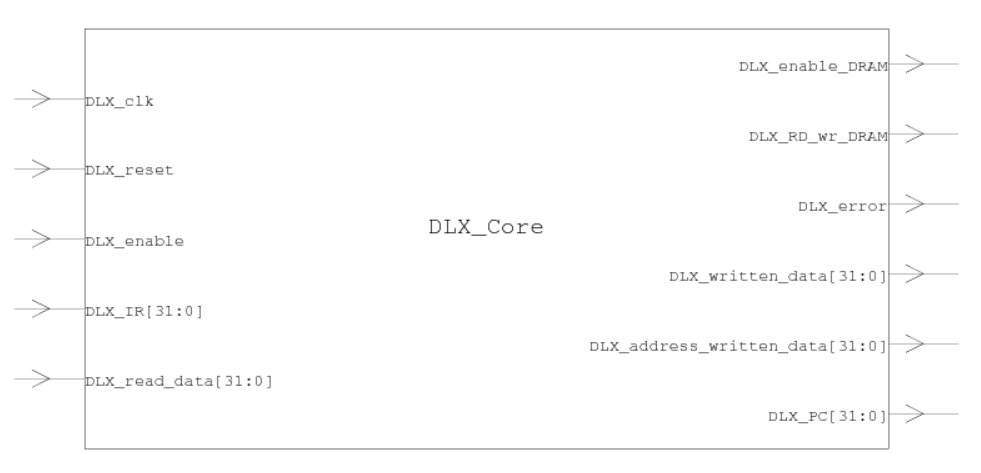
\includegraphics[scale=.6]{Immagini/05}
\label{02}
\caption{Core pinout}
\end{figure}

Just two informations about these signals. \textit{Clk} and \textit{enable} own their basic functionalities, \textit{IR} is the data read from the instruction RAM at each clock cycle by fetching. \textit{Read\_data} comes from the DRAM; \textit{enable\_DRAM} allows read and write operation on it, where the choice is made by \textit{RD\_wr\_RAM}. \textit{Error} is just a single pin out used for debugging, so not consider it. \textit{Written\_data} and \textit{address\_written\_data} are signals to the DRAM; in the end the \textit{PC} to the IRAM. \newline
The core is composed by 4 macroblocks:
\begin{itemize}
\item Datapath
\item Control unit
\item Branch target buffer
\item Branch misprediction manager
\end{itemize}
\begin{figure}[H]
\centering
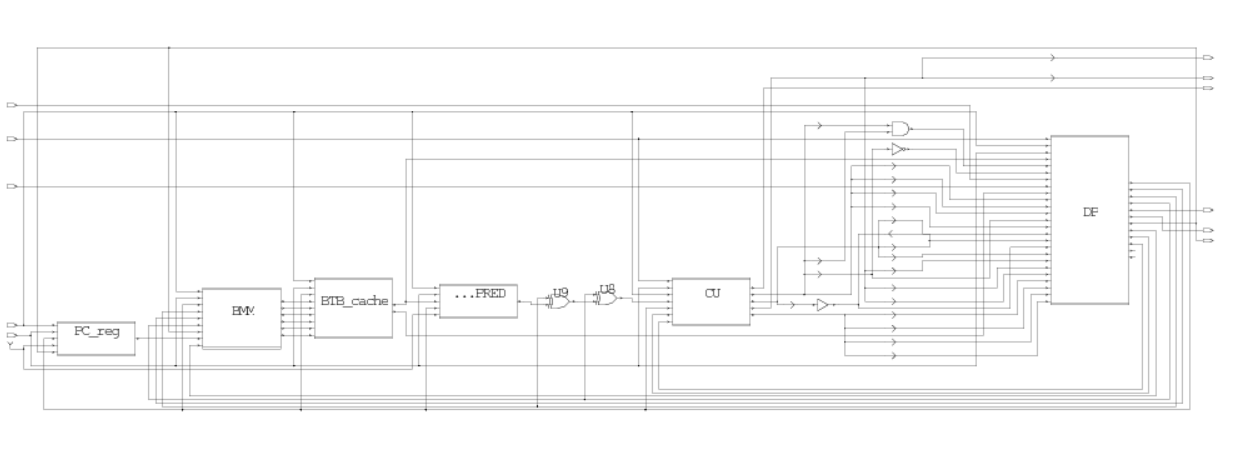
\includegraphics[scale=.6]{Immagini/06}
\label{02}
\caption{Core schematic - I}
\end{figure}

\begin{figure}[H]
\centering
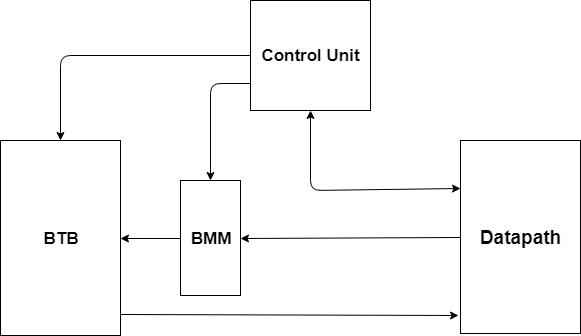
\includegraphics[scale=.6]{Immagini/07}
\label{02}
\caption{Core schematic - II}
\end{figure}
The datapath is the part of microprocessor computing instructions. In this design is the biggest component, where are defined the five pipeline stages. The branch target buffer is a sort of cache memory, used to manage control hazards; in fact branch addresses are stored in it. However almost all communications between datapath and BTB are managed by the Branch Misprediction Manager, which works when a wrong prediction occurs. Finally there is the hardwired Control Unit, that is the main brain of the DLX; as the datapath it's pipelined too.\newline
Datapath sends to BMM, so to BTB, information about the current instruction and the previous one such as: the program counter and whether one instruction is a branch or not. On the other side the BTB responds sending the branch target and the boolean value of the prediction (taken or untaken). The control unit oversees all macroblocks. It receives the instruction register of the instruction getting in the decode stage and produces all control signals.

\section{BTB}

I guess talking about BTB before datapath should let you understand better the overall behaviour of this microprocessor. Basically a Branch Target Buffer behaves like a cache. It's composed of a set of rows, where each rows defines three fields :
\begin{itemize}
\item Entry
\item Target
\item Status of prediction
\end{itemize}

The entry is basically the value of the PC related to the branch instruction. The target stands for the address to jump if that branch is taken. The status is held by a saturation counter, where the most significant bit defines the kind of prediction. In this design, this component has 32 entry 32 bits long, as well as the PC, the same for the target. Saturation counters count on 3 bits. 
\begin{figure}[H]
\centering
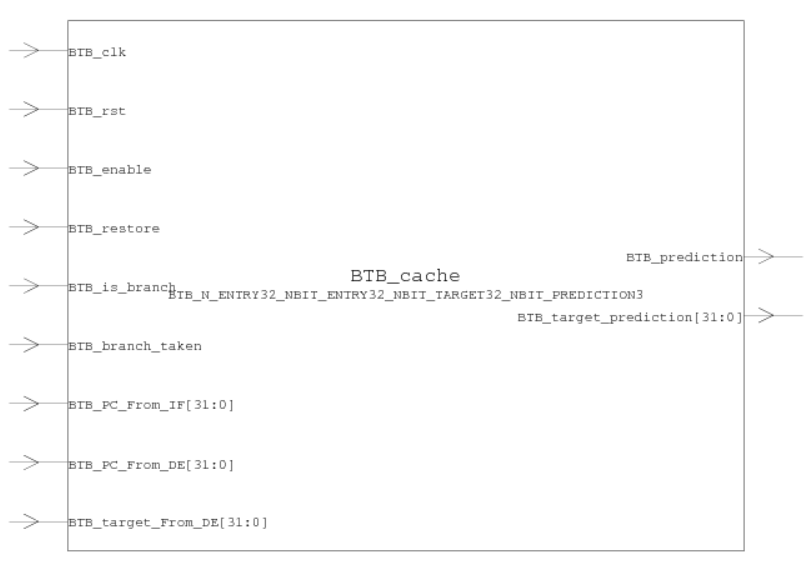
\includegraphics[scale=.7]{Immagini/08}
\label{02}
\caption{BTB pinout}
\end{figure}

Now it's important to focus on the meaning of each signals and understand the timing
\begin{table}[H]
\centering
\begin{tabular}{|p{0.3\textwidth}|p{0.2\textwidth}|p{0.1\textwidth}|p{0.4\textwidth}|}
\hline
\textbf{Signal}&\textbf{From}&\textbf{To}&\textbf{Note}\\ \hline
BTB\_enable & Control Unit & - & Active high. It gets low because of stalls\\ \hline
BTB\_is\_branch & Datapath->BMM & - & It is generated during the decode stage. It's high when the instruction is a branch, low otherwise\\ \hline
BTB\_restore & Datapath->BMM & - & When a bad prediction is given, it's needed to restore the previous status of prediction\\ \hline
BTB\_branch\_taken & Datapath->BMM & - & It's generated by decode stage. Regardless of kind of instruction and prediction, it provides a correct information on any kind of change of context. This signal is used by BTB to update the SAT\\ \hline
\end{tabular}
\caption{BTB signals I}
\end{table}
\begin{table}[H]
\centering
\begin{tabular}{|p{0.3\textwidth}|p{0.2\textwidth}|p{0.1\textwidth}|p{0.4\textwidth}|}
\hline
\textbf{Signal}&\textbf{From}&\textbf{To}&\textbf{Note}\\ \hline
BTB\_PC\_from\_IF & Datapath->BMM & - & It's the value of the PC of the instruction at fetching. It's sent to BTB immediately, so in case of hit, the predicted PC is granted back at the next clock cycle, without wasting time\\ \hline
BTB\_PC\_from\_DE & Datapath->BMM & - & It's the value of the PC of the branch instruction at decoding. It's used just in case of miss to store the new entry. It usually has the same value of BTB\_PC\_from\_IF at the next cc\\ \hline
BTB\_target\_from\_DE & Datapath->BMM & - & It's the value of the target to be jumped of the branch at decoding. It's used just in case of miss to store the new target. \\ \hline
BTB\_prediction & - & Datapath & True: prediction taken. False, otherwise \\ \hline
BTB\_target\_prediction & - & Datapath & New PC to be loaded in the fetch PC register \\ \hline
\end{tabular}
\caption{BTB signals II}
\end{table}

Look at the following code, which exploits the branch target buffer and analyse what happens inside. After the instruction is reported the address where it's stored in the IRAM.

\begin{lstlisting}[caption={Branch.asm}]
 nop				;0
 nop 				;4
 addi r1, r0, 100	;8
 xor r2, r2, r2		;12

 ciclo:
 lw r3, 0(r2)		;16
 addi r3, r3, 10	;20
 sw 100(r2), r3		;24
 subi r1, r1, 1		;28
 addi r2, r2, 4		;32
 bnez r1, ciclo		;36
					
					   
 addi r4, r0, 65535 ;40
 ori r5, r4, 100000	;44
 add r6, r4, r5		;48

 end:								
 j end				;52
\end{lstlisting}
\paragraph{Miss}
$\\$
$\\$
The first main event occurs at 125 ns, when the \lstinline{bnez} instruction is fetched. You can see PC\_from\_IF is 36, the previous PC instruction in decode, PC\_from\_de is 32; all entries and targets are empty. The saturation counter in the pictures is related to the first entry, others else are not reported, since they aren't used in this example. At 135 ns the fetched instruction is the \lstinline{addi}, but here the DLX is already wasting time, because we know that \lstinline{bnez} is taken. However, PC\_from\_de and Target\_from\_de report all significant data of the branch instruction; moreover, the decode stage provide BTB also the information that \lstinline{bnez} is a branch instruction and that it'has been a real taken. These data are stored by BTB: PC\_from\_de among entries, Target\_from\_de among targets and finally the saturation counter is set to 100.  \newline
If the set of rows is full the replacement policy adopted is the \textbf{first in first out}, implemented by means of a rotate register.
\paragraph{Hit}
$\\$
$\\$
At 205 ns \lstinline{bnez} is fetched again. Immediately BTB matches and sends out the prediction and target. This lead an advantage because at 215 ns the PC is 16, rather than 40. No clock cycles are lost. Concurrently the saturation counter increases by 1, strengthening the taken status.

\begin{figure}[H]
\centering
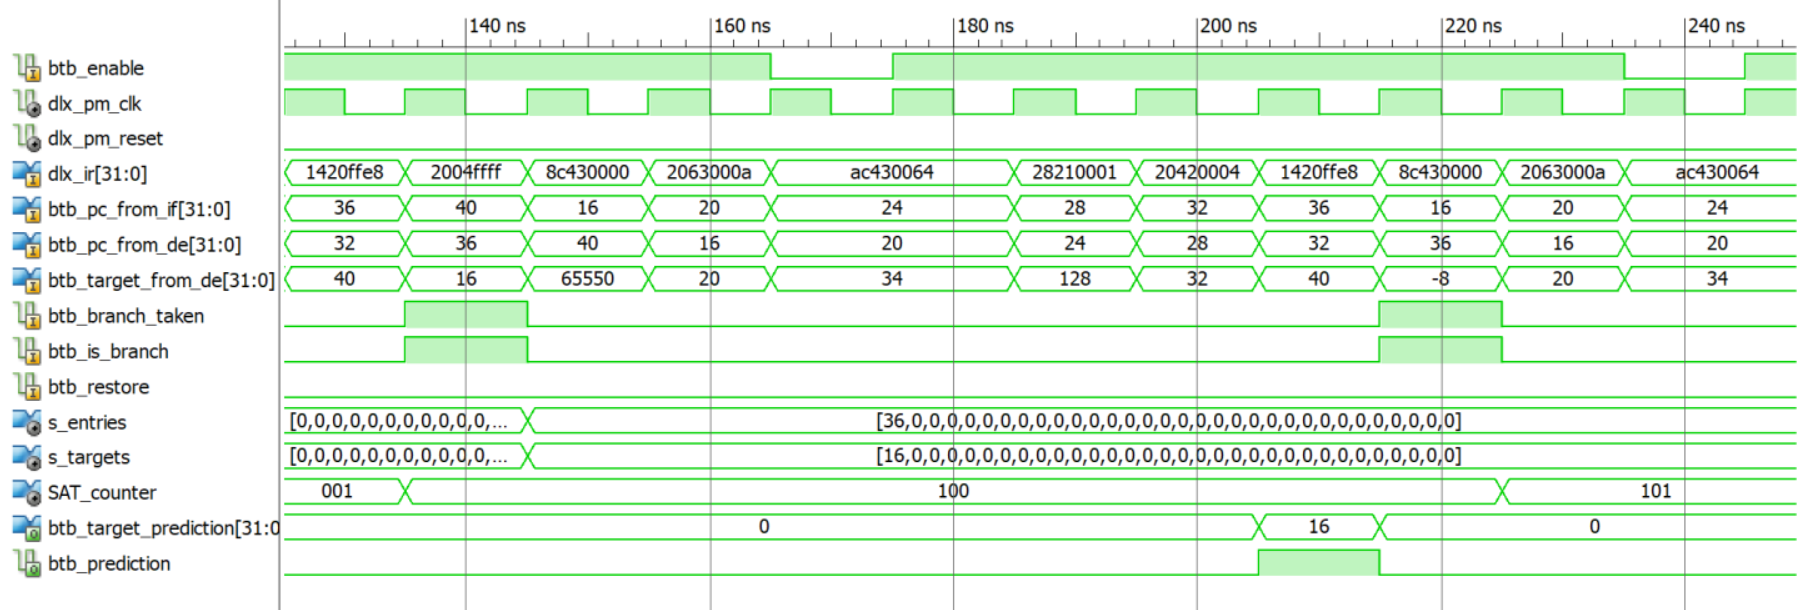
\includegraphics[scale=.4]{Immagini/09}
\label{09}
\caption{BTB waveform I}
\end{figure}

\paragraph{Restoring}
$\\$
$\\$
Execution goings on until the last iteration. At 7065 ns \lstinline{bnez} is fetched, BTB predicts taken. At 7075 ns the PC is updated to the target value, but decode stage recognizes the error and the datapath grants the restore signal. Remember that between BTB and datapath there is the Branch Misprediction Manager, which runs in transparent mode when everything is OK, but it gets working when a restore of the BTB is required. BMM recovers the entry and the target of the instruction with a wrong prediction, then for 2 clock cycles it keeps them at the BTB input. The same procedure works with Is\_branch and Branch\_taken signal; the latter is negated by BMM. Restoring protocol is used to fix the saturation counter content. Let's consider $\phi_1$ as the current value of the saturation counter.
\begin{enumerate}
\item BTB sends out prediction, here taken
\item Taken prediction makes $\phi_2=\phi_1+1$: actually no branch is taken
\item Restoring triggers. First cycle $\phi_3 = \phi_2-1$, it's a backtrack
\item Second restoring cycle $\phi_4 = \phi_3-1$, saving the correct and updated status
\end{enumerate}

Finally $\phi_4 = \phi_1-1$. The reason why I choose 3 bits follows. Let's consider a weak taken $\phi_1 = 10_2$, but branch untaken, so at the end $\phi_4 = 01_2$ a weak untaken, here everything works well. Now let's take into account a strong taken $\phi_1 = 11_2$, but branch untaken, at the end we get $\phi_4 = 01_2$, $\phi_2$ saturates to $11_2$ and at the end of the procedure we'd have a weak untaken: that's not make any sense. Adding a third bit overrides this issue and from a strong taken the status moves to a weak one: $\phi_1 = 111_2 \rightarrow \phi_2 = 111_2 \rightarrow \phi_3  = 110_2 \rightarrow \phi_4 = 101_2$

\begin{figure}[H]
\centering
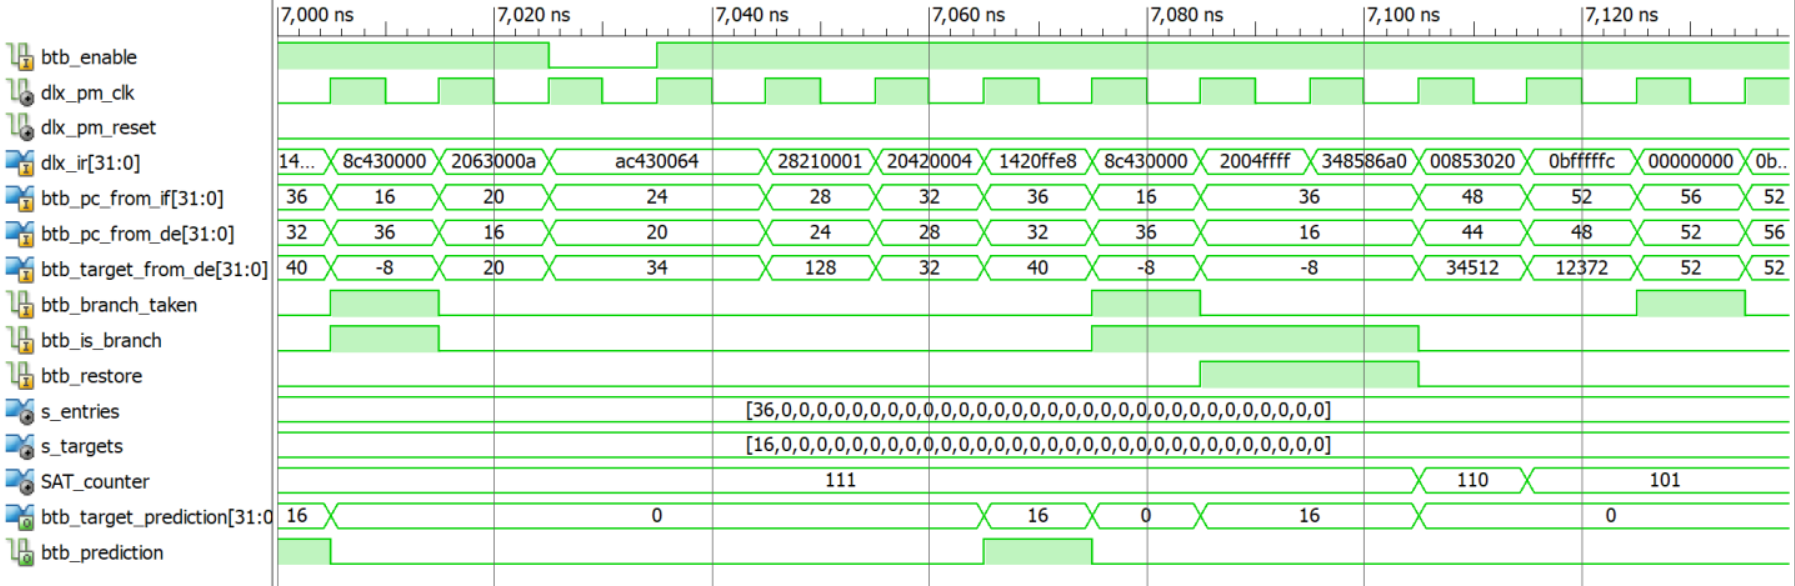
\includegraphics[scale=.4]{Immagini/10}
\label{10}
\caption{BTB waveform II}
\end{figure}
Main components making up the Branch Target Buffer are
\begin{itemize}
\item 32 Comparators (just check eq.)
\item 1 Priority Encoder
\item 64 Registers 32 bits
\item 1 Rotate register
\item 32 Saturation counters
\end{itemize}
\begin{figure}[H]
\centering
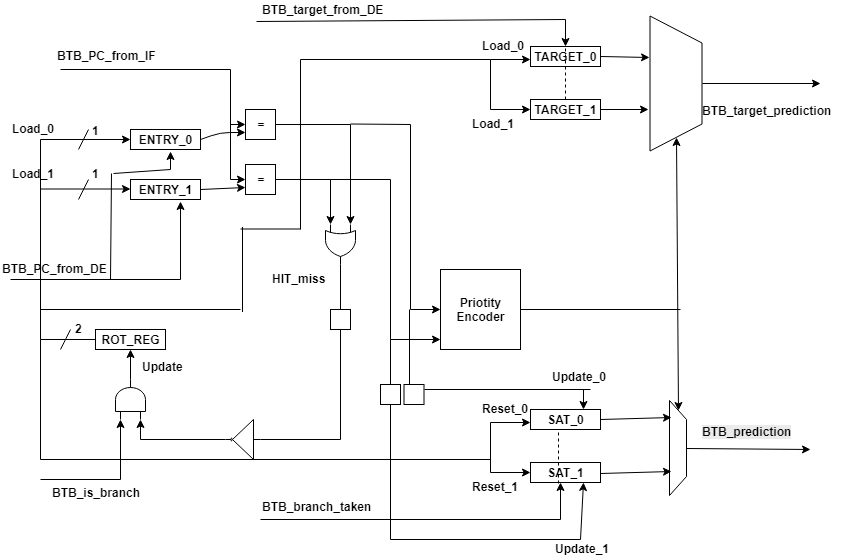
\includegraphics[scale=.5]{Immagini/11}
\label{11}
\caption{BTB simplyfied microarchitecture}
\end{figure}

\subsection{Comparator with enable}
This component matches the entries with the value of the PC. Further usual inputs I added the enable in order to avoid errors due to combinational logic, when the BTB is off.
\begin{figure}[H]
\centering
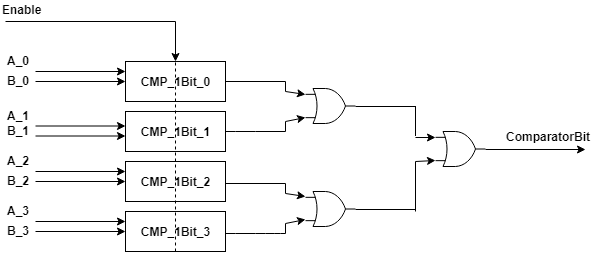
\includegraphics[scale=.7]{Immagini/12}
\label{12}
\caption{Comparator 4 bits schematic}
\end{figure}
As you can see, this component has 2 areas. The former is a set of 1-bit comparator, the latter is a pyramid of OR gates, in order to compute the final result: true equal, false unequal. \newline
Deeper, the 1-bit comparator has the following structure:
\begin{figure}[H]
\centering
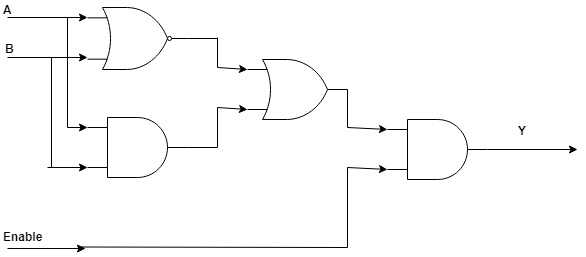
\includegraphics[scale=.7]{Immagini/13}
\label{13}
\caption{Comparator 1 bit schematic}
\end{figure}
\begin{table}[H]
\centering
\begin{tabular}{|p{0.1\textwidth}|p{0.1\textwidth}|p{0.1\textwidth}|p{0.1\textwidth}|}
\hline
\textbf{A}&\textbf{\textbf{B}}&\textbf{Enable}&\textbf{Y}\\ \hline
0 & 0 & 0 & 0\\ \hline
0 & 0 & 1 & 1\\ \hline
0 & 1 & 0 & 0\\ \hline
0 & 1 & 1 & 0\\ \hline
1 & 0 & 0 & 0\\ \hline
1 & 0 & 1 & 0\\ \hline
1 & 1 & 0 & 0\\ \hline
1 & 1 & 1 & 1\\ \hline

\end{tabular}
\caption{Comparator 1 bit truth table}
\end{table}

\subsection{Rotate register}
The BTB exploits a rotate register in order to implement the replacement policy (\cite{EFESbook}) First In First Out. This technique requires a pointer which is updated in case of a miss; the role of the pointer is covered by the rotate register output. When the BTB is resetted all the content of the rotate register is set to 0, except for the most significant bit to 1; moreover is never possible to load new data inside. It means that just reset, rotate (by 1) and keeping are allowed. That single bit to 1 is the pointer I'm referring to.

\begin{figure}[H]
\centering
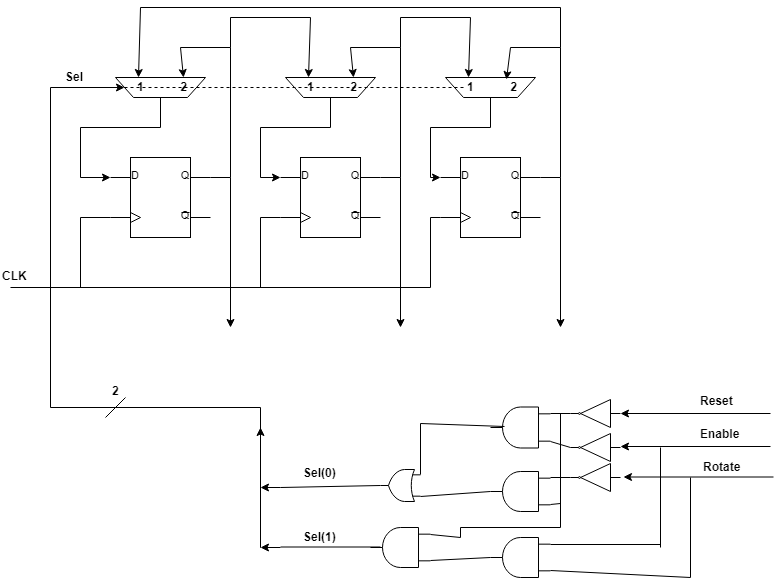
\includegraphics[scale=.6]{Immagini/14}
\label{14}
\caption{Rotate register schematic}
\end{figure}

\begin{table}[H]
\centering
\begin{tabular}{|p{0.1\textwidth}|p{0.1\textwidth}|p{0.1\textwidth}|p{0.2\textwidth}|}
\hline
\textbf{Reset}&\textbf{\textbf{Enable}}&\textbf{Rotate}&\textbf{Sel}\\ \hline
0 & 0 & 0 & 10 Keep\\ \hline
0 & 0 & 1 & 10 Keep\\ \hline
0 & 1 & 0 & 10 Keep\\ \hline
0 & 1 & 1 & 01 Rotate\\ \hline
1 & - & - & 00 Reset\\ \hline

\end{tabular}
\caption{Multiplexer selector  truth table}
\end{table}

\subsection{Saturation counter}
A saturation counter is a finite state machine which behavies like a usual counter, implementing up and down operation, but the difference is that it cannot get either overflow or underflow. 
\begin{figure}[H]
\centering
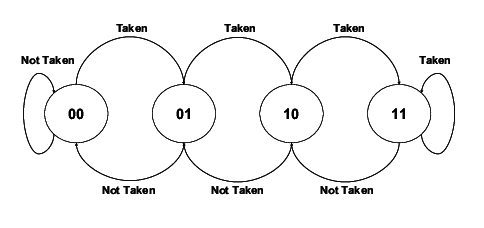
\includegraphics[scale=.8]{Immagini/15}
\label{15}
\caption{2-bit SAT counter FSM}
\end{figure}
The usual architecture of a FSM is composed of a control unit and a datapath. This components ows this structure, where the role of the datapath is covered by a UpDownCounter, which is not a saturation one. The UDCounter can get overflow and underflow. On the other side the control unit checks the status of the datapath in order to stall the counting in case an Up is required when has been already reached the maximum, or a Down has to be performed when has been already hit the minimum value.
\begin{figure}[H]
\centering
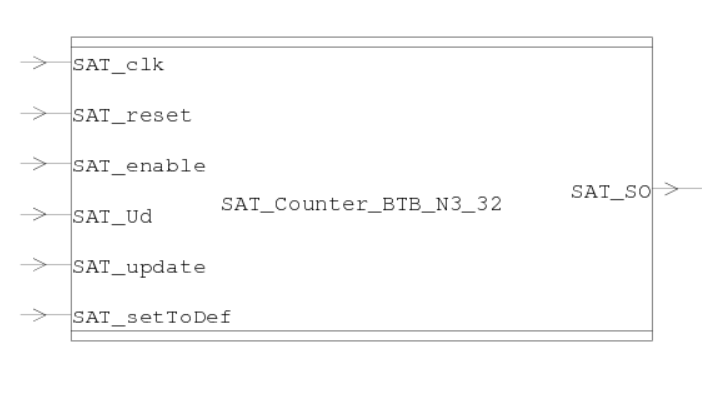
\includegraphics[scale=.8]{Immagini/16}
\label{16}
\caption{SAT counter pinout}
\end{figure}

\begin{figure}[H]
\centering
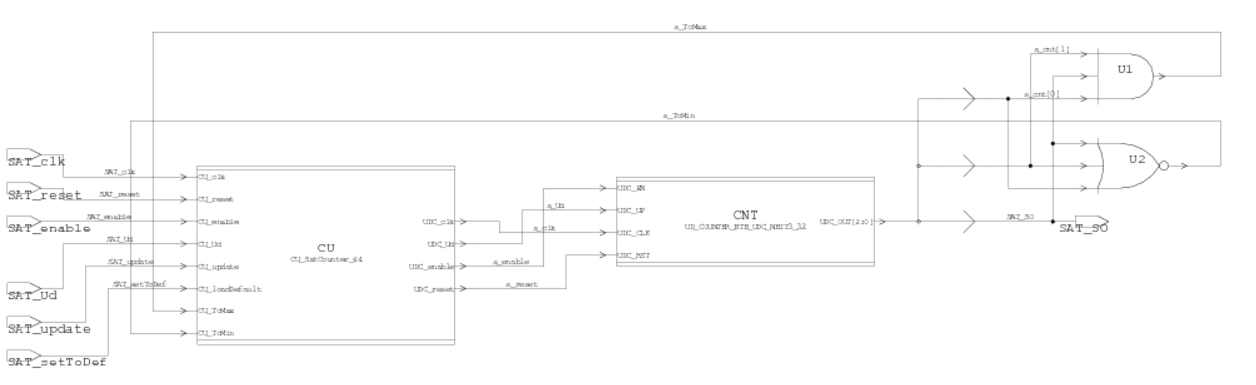
\includegraphics[scale=.6]{Immagini/17}
\label{17}
\caption{SAT counter microarchitecture}
\end{figure}

From the VHDL point of view, the control unit owns a behavioral description, the UDCounter a structural one, built with TFF. Since I designed a reset value equals to a weak taken status (MSB = '1', others '0'), two versions of FF are used, where the difference is just the value to load into when reset signal is triggered.\newline
The most significant bit is used as predictor. 


\section{BTB misprediction manager}
The BTB misprediction manager is the interface between datapath and BTB. This component is totally original, I didn't get inspired from anything, I designed just functionalities I needed. \newline
It has two operative modes:
\begin{itemize}
\item \textbf{Transparent} : Signals go from datapath to branch target buffer without incurring any penalties
\item \textbf{Restoring} : Data are managed in order to recover the correct status of the saturation counter of the entry having been predicted in a wrong way
\end{itemize}

\begin{figure}[H]
\centering
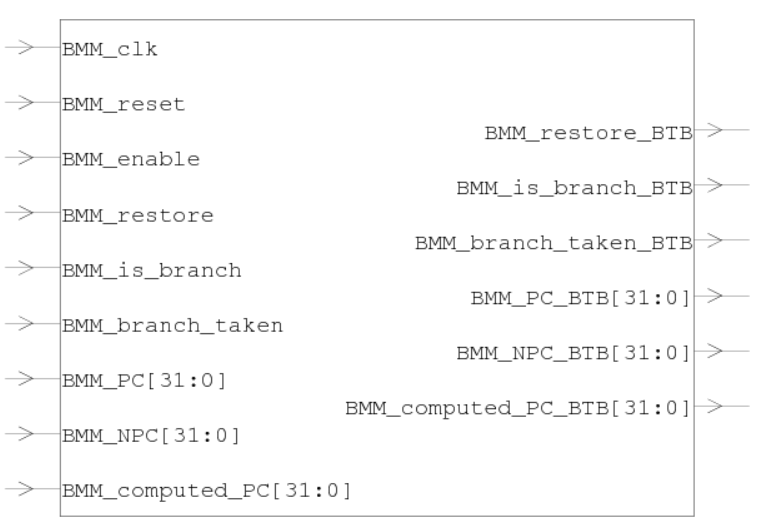
\includegraphics[scale=.7]{Immagini/18}
\label{18}
\caption{BMM pinout}
\end{figure}
\begin{table}[H]
\centering
\begin{tabular}{|p{0.3\textwidth}|p{0.2\textwidth}|p{0.1\textwidth}|p{0.3\textwidth}|}
\hline
\textbf{Signal}&\textbf{From}&\textbf{To}&\textbf{Note}\\ \hline
BMM\_enable & Control Unit & - & Active high. It gets low because of stalls \\ \hline
BMM\_restore &  Datapath & - & When a bad prediction is given, it's needed to restore the previous status of prediction. When 1 triggers \textbf{restoring mode}, 0 keeps \textbf{transparent}\\ \hline
BMM\_is\_branch & Datapath & - & It is generated during the decode stage. It's high when the instruction is a branch, low otherwise\\ \hline
BMM\_branch\_taken & Datapath & - & It's generated by decode stage. Regardless of kind of instruction and prediction, it provides a correct information on any kind of change of context\\ \hline
BMM\_PC & Datapath & - & It's the value of the PC of the instruction at fetching. \\ \hline
BMM\_NPC & Datapath & - & It's the value of the PC of the branch instruction at decoding.\\ \hline
BMM\_computed\_PC & Datapath & - & It's the value of the target to be jumped of the branch at decoding. \\ \hline
BMM\_restore\_BTB & - & BTB & Read BMM\_restore\\ \hline
BMM\_is\_branch\_BTB & - & BTB & Read BMM\_is\_branch  \\ \hline
BMM\_branch\_taken\_BTB & - & BTB & Read BMM\_branch\_taken \\ \hline
BMM\_PC\_BTB & - & BTB & Read BMM\_PC\\ \hline
BMM\_NPC\_BTB & - & BTB & Read BMM\_NPC\\ \hline
BMM\_computed\_PC\_BTB & - & BTB & Read  BMM\_computed\_PC \\ \hline
\end{tabular}
\caption{BMM signals}
\end{table}
\paragraph{Transparent}
$\\$
$\\$
Signals go through BMM when BMM\_restore is 0, without wasting times.

\paragraph{Restoring}
$\\$
$\\$
It triggers when BMM\_restore goes to 1. It actives a saturation counter computing just down steps. That 2-bit counter starts from a value of 10. The output is connected to a XOR gate, whose result is 1 when the 2 input bits are not equal. This logical gate produces the enable, then negated, for registers, that will store all data coming from datapath; moreover the output multiplexers will switch to the input port wired to those registers outputs. As you can understand, the restoring mode lasts 2 clock cycle,  the BMM output is driven to freezed values. Concurrently the register enable is kept to 0, by XNORing, for all the duration of this procedure. \newline
BMM\_restore is driven to 1, by datapath, just for 1 clock cycle (not 2), this means that it's possible the scenario where restoring is running and BMM\_restore is 0. \newline
The BMM microarchitecture is pretty regular, a small excpetion for BMM\_branch\_taken connections. Its register gets as input the negated value. In fact, when restoring procedure triggers a wrong prediction occured, so BTB has to receive the opposite branch (real) condition. 

\begin{figure}[H]
\centering
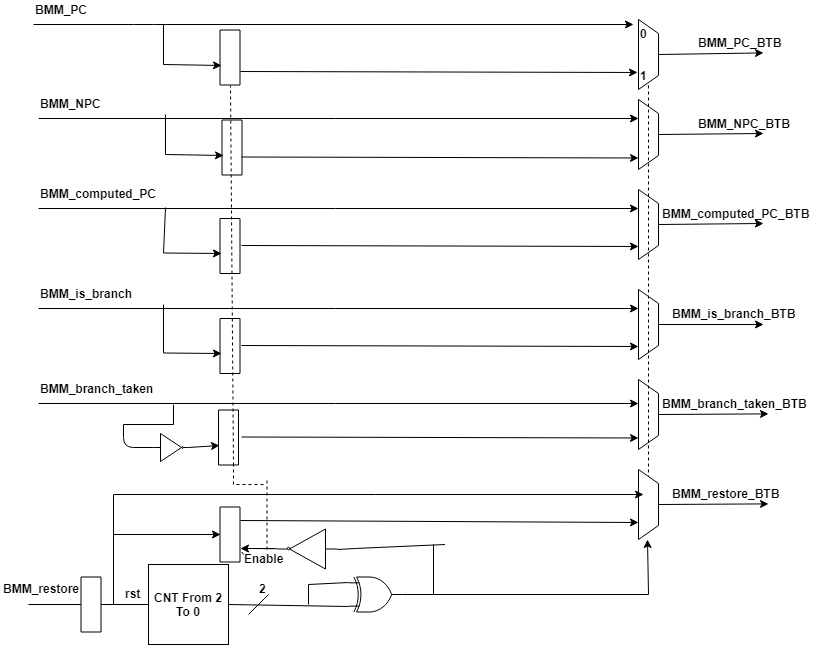
\includegraphics[scale=.5]{Immagini/19}
\label{19}
\caption{BMM microarchitecture}
\end{figure}

